\documentclass{beamer}
\usepackage{amsfonts,amsmath,oldgerm}
\usepackage{natbib}
\usetheme{sintef}

\newcommand{\testcolor}[1]{\colorbox{#1}{\textcolor{#1}{test}}~\texttt{#1}}

\usefonttheme[onlymath]{serif}

\titlebackground*{assets/background}

\newcommand{\hrefcol}[2]{\textcolor{cyan}{\href{#1}{#2}}}

\title{Computação, Infoproletariado e Liberdade Digital}
\subtitle{Ciclo de Formações do Patos à Esquerda}
\author{\href{mailto:viniciusmacielf@gmail.com}{Vinícius Fonseca Maciel}}
\date{2023}

\begin{document}
\maketitle

\begin{frame}{Licença de Uso}
	\framesubtitle{Licença de Uso}
	\begin{block}{Documento sob a licença GFDL}
		Copyright (c)  2024  Vinícius F. Maciel. \\ Permission is granted to copy, distribute and/or modify this document under the terms of the GNU Free Documentation License, Version 1.3 or any later version published by the Free Software Foundation; with no Invariant Sections, no Front-Cover Texts, and no Back-Cover Texts. A copy of the license is included in the section entitled "GNU Free Documentation License".
	\end{block}
\end{frame}

\section{Computação e Software Livre}

\begin{frame}{Computação}
    \begin{itemize}
        \item A computação integra as bases da estrutura capitalista e ela é oportunamente utilizada no controle das massas.
        \item A militância da esquerda revolucionária anticapitalista precisa compreender o universo digital.
        \item Compreender significa poder estudar e contestar/creditar as configurações sociais que surgem a partir da evolução tecnológica.
    \end{itemize}
\end{frame}

\begin{frame}{Computação}
    \begin{itemize}
        \item Alguns conceitos importantes sobre computação:
        \begin{itemize}
            \item Algoritmos
            \item Programa
            \item Linguagem de programação e código-fonte
            \item Código de máquina
            \item Sistemas Operacionais
        \end{itemize}
    \end{itemize}
\end{frame}

\begin{frame}{Computação | Algoritmos}
    \begin{columns}
        \begin{column}{0.5\textwidth}
            \begin{figure}
                \centering
                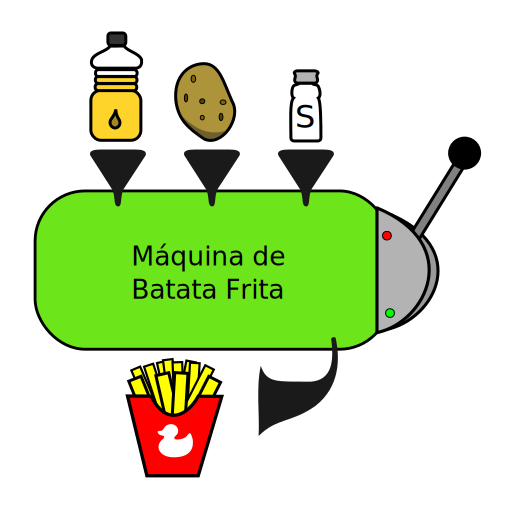
\includegraphics[width=0.7\linewidth]{img/maquina-de-batata.png}
                \caption{Uma máquina de fazer batata frita}
                \label{fig:enter-label}
            \end{figure}
        \end{column}
        \begin{column}{0.5\textwidth}
            \begin{itemize}
                \item \textbf{Algoritmo}: sequência finita de passos que levam à resolução de um problema.
                \item \textbf{Problema}: fazer uma batata frita.
                \item Um algoritmo, informalmente, pode ser interpretado neste contexto como uma ``\textbf{receita}''.
                \item \textbf{Qual é a receita?}
            \end{itemize}
        \end{column}
    \end{columns}
\end{frame}

\begin{frame}{Computação | Algoritmos}
    \begin{itemize}
        \item Para construir algoritmos usamos um conceito fundamentalmente utilizado na orquestração lógica de nossas sinapses em basicamente tudo que fazemos. São elas duas coisas: um conjunto histórico de dados e uma definição de sucesso.
        \item Na computação usamos a clássica sequência para definir o funcionamento de um algoritmo: $ Entrada \rightarrow Processamento \rightarrow Saida$
    \end{itemize}
\end{frame}

\begin{frame}{Computação | Programa}
    \begin{itemize}
        \item A tradução do algoritmo para um formato em que uma entidade seja capaz de executá-lo define um \textbf{programa}.
        \item Descobrir o M.M.C. pode se constituir de um mesmo algoritmo tanto para o humano quanto para uma máquina, o que diferencia é a ``linguagem" utilizada por eles.
        \item Software, aplicação, aplicativo e programa de computador são termos similares sensíveis ao contexto.
    \end{itemize}
\end{frame}

\begin{frame}{Computação | Linguagem \& Código-fonte}
    \begin{itemize}
        \item Linguagem define um \textbf{conjunto de palavras} (léxico) que obedecem um \textbf{conjunto de regras} (sintaxe) a fim de \textbf{definir um sentido} (semântica).
        \item A \textbf{linguagem} entendida por um computador é \textbf{artificial}, formalmente definida na matemática.
        \item Ser um programador de computadores exige a compreensão da linguagem utilizada na escrita de um programa.
        \item O código-fonte é um arquivo construído com textos redigidos a partir do uso destas linguagens para formar o software.
    \end{itemize}
\end{frame}

\begin{frame}{Computação | Linguagem \& Código-fonte}
    \begin{itemize}
        \item Linguagens de programação
    \end{itemize}
    \begin{figure}
        \centering
        \includegraphics[width=0.8\linewidth]{img/prog-languages.png}
    \end{figure}
\end{frame}

\begin{frame}{Computação | Linguagem \& Código-fonte}
    \begin{itemize}
        \item Este é um exemplo de programa, chamado ``Greetings'' escrito em Python.
        \item Python é uma linguagem de muito alto nível, em outras palavras, bastante amigável
    \end{itemize}
    \begin{figure}
        \centering
        \includegraphics[width=0.7\linewidth]{img/greetings-code/greetings-python.png}
        \caption{Código em Python}
    \end{figure}
\end{frame}

\begin{frame}{Computação | Linguagem \& Código-fonte}
    \begin{itemize}
        \item Esta é a execução do programa ``Greetings".
        \item O usuário preencheu seu nome (entrada) e recebeu uma mensagem ``Olá, Vinícius Maciel" (saída).
    \end{itemize}
    \begin{figure}
        \centering
        \includegraphics[width=0.7\linewidth]{img/greetings-code/greetings-terminal.png}
        \caption{Execução de programa}
    \end{figure}
\end{frame}

\begin{frame}{Computação | Linguagem \& Código-fonte}
    \begin{itemize}
        \item Quanto menor o ``nível'' da linguagem, mais ``difícil'' pode ser sua compreensão humana, porém mais ``fácil'' para o computador.
        \item Próximo: mesmo programa escrito na linguagem C (médio nível)
    \end{itemize}
\end{frame}

\begin{frame}{Computação | Linguagem \& Código-fonte}
    \begin{figure}
        \centering
        \includegraphics[width=0.4\linewidth]{img/greetings-code/greetings-c.png}
    \end{figure}
\end{frame}

\begin{frame}{Computação | Linguagem \& Código-fonte}
    \begin{itemize}
        \item Próximo: mesmo programa escrito na linguagem NASM, que é um tipo de Assembly (baixo nível)
    \end{itemize}
\end{frame}

\begin{frame}{Computação | Linguagem \& Código-fonte}
    \begin{figure}
        \centering
        \includegraphics[width=0.4\linewidth]{img/greetings-code/greetings-nasm-0.png}
    \end{figure}
\end{frame}
\begin{frame}{Computação | Linguagem \& Código-fonte}
    \begin{figure}
        \centering
        \includegraphics[width=0.4\linewidth]{img/greetings-code/greetings-nasm-1.png}
    \end{figure}
\end{frame}
\begin{frame}{Computação | Linguagem \& Código-fonte}
    \begin{figure}
        \centering
        \includegraphics[width=0.4\linewidth]{img/greetings-code/greetings-nasm-2.png}
    \end{figure}
\end{frame}

\begin{frame}{Computação | Linguagem \& Código-fonte}
    \begin{itemize}
        \item Próximo: linguagem de máquina (código binário)
    \end{itemize}
\end{frame}

\begin{frame}{Computação | Código de Máquina}
    \begin{figure}
        \centering
        \includegraphics[width=0.6\linewidth]{img/greetings-code/greetings-bin.png}
    \end{figure}
\end{frame}

\begin{frame}{Computação | Código de Máquina}
    \begin{itemize}
        \item O computador entende apenas as \textbf{instruções binárias}.
        \item \textbf{Compilador}: As outras linguagens (assembly, médio e alto nível) são \textbf{traduzidas} para conjuntos de valores binários.
        \item É possível, com dificuldade, \textbf{reverter} estes valores binários para uma linguagem de maior alto nível e assim \textbf{tentar} reproduzir um código-fonte próximo do original. 
    \end{itemize}
\end{frame}

\begin{frame}{Computação | Código de Máquina}
    \begin{itemize}
        \item \textbf{Problema}: compiladores deixam o código mais ``bagunçado'', isso torna difícil o trabalho de \textbf{engenharia reversa}. 
        \item Este problema, entretanto, é \textbf{conveniente para os distribuidores de software proprietário}.
    \end{itemize}
    \begin{figure}
        \centering
        \includegraphics[width=0.25\linewidth]{img/evil-apple.jpg}
    \end{figure}
\end{frame}

\begin{frame}{Computação | Sistemas Operacionais}
    \begin{itemize}
        \item O sistema operacional é um software especial que \textbf{controla o acesso} de outros softwares aos recursos oferecidos pelo computador: processadores, memória, unidades de armazenamento, periféricos...
        \item Permite com que \textbf{programas executem concomitantemente}: você consegue ouvir música enquanto escreve um documento.
        \item Sem os sistemas operacionais, os computadores são inúteis.
    \end{itemize}
\end{frame}

{
\setbeamertemplate{navigation symbols}{}
\begin{frame}[plain]
    \makebox[\linewidth]{\includegraphics[width=\paperwidth]{img/sistemas-operacionais.png}}
\end{frame}
}

\begin{frame}{Software \textbf{Não} Livre}
    \begin{itemize}
        \item Todo software pode ter como meio de distribuição sua versão ``pronta'', i.e. compilada, para o funcionamento nos computadores.
        \item Houve um tempo em que se comprava o hardware e, como \textbf{``brinde''}, vinham os softwares juntos ao código-fonte para que o usuário pudesse \textbf{modificar}.
        \item Comunidade de usuários de computador era pequena. Era comum programadores escreverem códigos para seus equipamentos e \textbf{compartilhá-los entre universidades e corporações}. (\cite{RTC2009})
    \end{itemize}
\end{frame}

\begin{frame}{Software \textbf{Não} Livre}
    \begin{itemize}
        \item Martin Goetz registra a \textbf{primeira patente de software} em 19 de junho de 1968 (\cite{torres2013}) 
        \item IBM \textbf{inova} na cobrança separada de recursos em 23 de junho 1969. (\cite{johnson1998})
    \end{itemize}
    \begin{figure}
        \centering
        \includegraphics[width=0.4\linewidth]{img/Computerworld.png}
    \end{figure}
\end{frame}

\begin{frame}{Software \textbf{Não} Livre}
    Alguns efeitos da falta de liberdade:
    \begin{columns}
        \begin{column}{0.8\textwidth}
            \begin{itemize}
                \item A clássica luta contra os \textbf{gerenciadores de direitos digitais} (DRM).
                \begin{itemize}
                    \item Restrições de cópia, geolocalização, integridade do dispositivo, versões obrigatórias, ... (\cite{GNUDRM})
                \end{itemize}
                \item \textbf{Restrição} de aproveitamento de recurso físico por software.
                \begin{itemize}
                    \item ex. ``DLC'' de carro de luxo.
                \end{itemize}
                \item \textit{Spywares} e \textit{Backdoors} injetados \textbf{propositalmente}.
                \item \textbf{Roubo} de dados e \textbf{escravização} do usuário.
                \item A \textbf{obsolescência programada} via software.
            \end{itemize}
        \end{column}
        \begin{column}{0.2\textwidth}
            \begin{figure}
                \centering
                \includegraphics[width=1.2\linewidth]{img/control.png}
            \end{figure}
        \end{column}
    \end{columns}
\end{frame}

\begin{frame}{Software \textbf{Não} Livre}
    Alguns ``sabores'' da não liberdade:
    \begin{itemize}
        \item \textbf{Software proprietário/privativo}: qualquer software que não se tem acesso ao código-fonte, nem tem permissão de redistribuição gratuita.
        \item \textbf{Freeware}: permitem redistribuição gratuita. (sem código-fonte)
        \item \textbf{Shareware}: redistribuição permitida, e.g. trial/demo, mas necessita licença obrigatória. (sem código-fonte)
        \item \textbf{Softwares privados}: desenvolvido para um usuário específico, sem redistribuição. (este usuário \textit{pode} ter acesso ao código-fonte)
        \item \textbf{Software comercial}: Distribuição sob licenciamento de venda. É até possível vender uma distribuição de um software livre, e.g Red Hat. (\textit{pode} ou \textit{não} ter código-fonte)
    \end{itemize}
\end{frame}

\begin{frame}{Software Livre}
    \begin{block}{Liberdades}
        \begin{enumerate}
            \setcounter{enumi}{-1}
            \item A liberdade de \textbf{executar} o programa como você desejar, para qualquer propósito.
            \item A liberdade de \textbf{estudar} como o programa funciona, e adaptá-lo às suas necessidades. Para tanto, acesso ao código-fonte é um pré-requisito.
            \item A liberdade de \textbf{redistribuir} cópias de modo que você possa ajudar outros.
            \item A liberdade de \textbf{distribuir} cópias de suas versões modificadas a outros. Desta forma, você pode dar a toda comunidade a chance de beneficiar de suas mudanças. Para tanto, acesso ao código-fonte é um pré-requisito.
        \end{enumerate}
    \end{block}
\end{frame}

\begin{frame}{Software Livre}
    \begin{itemize}
        \item Se o \textbf{usuário tem todas as quatro liberdades} garantidas em um determinado software, aquele software é livre, e se o usuário se \textbf{compromete} a usar software livre, então ele é \textbf{livre} (\cite{RTC2009}).
        \item Ser um software ``de graça" não o torna um software livre.
        \item Hoje é possível usar um sistema computacional totalmente livre!
        \begin{itemize}
            \item Desde firmwares e gereciadores de boot até os softwares utilitários do dia a dia.
        \end{itemize}
    \end{itemize}
\end{frame}

\begin{frame}{Software Livre}
    \begin{itemize}
        \item ``O Software Livre é o primeiro movimento de luta pela \textbf{libertação do ciberespaço.}''
        \item Surgiu da \textbf{indignação} dos ``hackers'' do laboratório de IA do MIT nos anos 80. Em destaque: ``Richard Stallman".
        \item Os ``hackers'' do MIT eram conhecidos por quebrar a exclusividade de uso dos recursos computacionais da instituição e sempre conseguir \textbf{democratizar o acesso} ao que precisavam.
    \end{itemize}    
\end{frame}

\begin{frame}{Software Livre}
    \begin{columns}
        \begin{column}{0.7\textwidth}
            \begin{itemize}
                \item Symbolics monopoliza as máquinas Lisp do laboratório de IA do MIT e controla a atmosfera colaborativa da comunidade ``hacker''.
                \item Stallman em \textbf{retaliação à empresa Symbolics}, que decidiu acabar com o compartilhamento livre de códigos dentro do laboratório de IA, reprogramou todas as soluções da empresa e continuou compartilhando o código entre os seus. (\cite{RTC2009})
            \end{itemize} 
        \end{column}
        \begin{column}{0.3\textwidth}
            \begin{figure}
                \centering
                \includegraphics[width=1\linewidth]{img/220px-LISP_machine.jpg}
            \end{figure}
        \end{column}
    \end{columns}
\end{frame}

\begin{frame}{Software Livre}
    \begin{itemize}
        \item Quase todo software importante do meio da década de 80 é proprietário.
        \item Em 1985, Stallman lança o manifesto GNU e cria \textit{Free Software Foundation}(FSF).
        \item GNU desenvolve utilitários e desenvolve a casca (shell) que faz a interface usuário-sistema operacional.
        \item GNU = GNU's Not Unix
        \item Faltava o núcleo (\textit{kernel}) que integraria um Sistema Operacional completo.
    \end{itemize}
    \begin{figure}
        \centering
        \includegraphics[width=0.4\linewidth]{img/gnulinux.png}
    \end{figure}
\end{frame}

\begin{frame}{Software Livre | Linux}
    \begin{itemize}
        \item Linux (1991) é um núcleo de sistema operacional (\textit{kernel}), o termo correto para uma distribuição como Debian é GNU/Linux.
        \item Linux = ``Unix-like'' do Linus Torvalds. 
        \item O GNU/Linux é utilizado pela maioria das corporações ativas na internet como solução para servidores.
        \item Android possui o Linux como \textit{kernel}.
    \end{itemize}
\end{frame}

\begin{frame}{Software Livre | Linux}
    \begin{itemize}
        \item Linux e GNU possuem licença GPL, mas é constantemente contaminado e redistribuído com soluções proprietárias.
    \end{itemize}
    \begin{figure}
        \centering
        \includegraphics[width=0.5\linewidth]{img/nonfree.png}
    \end{figure}
\end{frame}

\begin{frame}{Software Livre | Licenças}
    Existem quatro tipos de licenças básicas que se originaram a partir do projeto GNU.
    \begin{itemize}
        \item \textbf{GNU GPL}: Licença Pública Geral - Aplicações
        \item \textbf{GNU LGPL}: Licença Pública Geral Menor - Bibliotecas de Software
        \item \textbf{GNU AGPL}: Licença Pública Geral Affero - Servidores
        \item \textbf{GNU FDL}:  Licença de Documentação Livre - Manuais e Documentos de Software
    \end{itemize}
    \begin{figure}
        \centering
        \includegraphics[width=0.8\linewidth]{img/licencas.png}
    \end{figure}
\end{frame}

{
\setbeamertemplate{navigation symbols}{}
\begin{frame}[plain]
    \makebox[\linewidth]{\includegraphics[width=\paperwidth]{img/logos2.png}}
\end{frame}
}

\begin{frame}{Software Livre - Críticas}
    \begin{itemize}
        \item \textbf{Opinião}: Forte em aspectos tecnológicos, frágil em aspectos políticos.
        \item Em \cite{torres2013}, evidencia-se uma \textbf{retórica neoliberal} submersa na estrutura da comunidade software livre.
        \item A \textit{open source initiative} é uma dissidência da comunidade software livre para ``amenizar'' o caráter combativo e se tornar \textbf{mais palatável para o mundo corporativo}.
        \item Autoritarismo, egocentrismo e elitismo tecnológico ainda permeiam os canais da comunidade.
    \end{itemize}
\end{frame}

\begin{frame}{Digitaliza}
    \begin{columns}
        \begin{column}{0.7\textwidth}
            \begin{itemize}
                \item Projeto de restaurações de dispositivos computacionais (\cite{VINIPAE}).
                \item Priorização de Softwares Livres e código-fonte aberto.
                \item \textbf{Sistemas legados lidam bem com o software livre}.
                \item É interessante para o projeto também a \textbf{recuperação de \textit{smartphones}}, entretanto a limitação fica a cargo do modelo e do tipo dos Androids Custom Roms.
            \end{itemize}
        \end{column}
        \begin{column}{0.3\textwidth}
            \begin{figure}
                \centering
                \includegraphics[width=1\linewidth]{img/digitaliza.png}
            \end{figure}
        \end{column}
    \end{columns}
\end{frame}

\section{Infoproletariado e Uberização}

\begin{frame}{Proletariado na era digital}
    \begin{itemize}
        \item Percepção da quebra de paradigma laboral: não existe mais o trabalhador sem um \textit{smartphone}.
        \item O \textbf{infoproletariado}, como termo, surge da compreensão de um novo subconjunto de tipos de trabalho que mesclam a tecnologia do século XXI e as condições de trabalho abusivas do século XIX. (\cite{antunes2009})
    \end{itemize}
\end{frame}

\begin{frame}{Proletariado na era digital}
    \begin{itemize}
        \item A indústria 4.0 acentua o uso das tecnologias da informação e comunicação (TIC). 
        \item A expansão do trabalho precarizado pelas TICs significará a \textbf{ampliação dos processos produtivos} ainda mais automatizados e robotizados em toda a cadeia de valor, de modo que a \textbf{logística empresarial será toda controlada digitalmente}. (\cite{antunes2020})
        \item Ampliação do trabalho morto.
    \end{itemize}
\end{frame}

\begin{frame}{Uberização}
    \begin{itemize}
        \item Mutação do \textit{Zero Hour Contract}: o trabalho é condicionado ao chamado de uma plataforma.
        \item O trabalhador ganha estritamente pelo que fizer, não recebe pelo \textbf{tempo que espera}.
        \item \textbf{Uberização}: as relações de trabalho são crescentemente \textbf{individualizadas} e \textbf{invisibilizadas}, assumindo a apareência de ``prestação de serviços'' e \textbf{obliterando as relações de assalariamento} e de exploração de trabalho. (\cite{antunes2020})
    \end{itemize}
\end{frame}

\begin{frame}{Breque dos Apps}
    \begin{columns}
        \begin{column}{0.7\textwidth}
            \begin{itemize}
                \item \textbf{Breque dos Apps}: Primeira grande mobilização grevista organizada por entregadores de aplicativos no Brasil. (01/07 e 25/07 de 2020)
                \item Clima de pandemia global e intensa precarização dos entregadores: pulou de 280 mil para 500 mil entregadores registrados.
                \item Entregadores Antifacistas, Paulo Galo e reivindicações:
                \begin{itemize}
                    \item Diminuição do valor por km rodado, diminuição da taxa mínima de entrega, fim dos bloqueios arbitrários, fim do sistema de pontuação, auxílio pandemia (EPI e auxílio saúde)
                \end{itemize}
            \end{itemize}
        \end{column}
        \begin{column}{0.3\textwidth}
            \begin{figure}
                \centering
                \includegraphics[width=1\linewidth]{img/Paulo_lima_galo.jpg}
            \end{figure}
        \end{column}
    \end{columns}
\end{frame}

\begin{frame}{Yuri Fontes}
    \begin{columns}
        \begin{column}{0.5\textwidth}
            \begin{figure}
                \centering
                \includegraphics[width=1\linewidth]{img/yuri.png}
            \end{figure}
        \end{column}
        \begin{column}{0.5\textwidth}
            \begin{figure}
                \centering
                \includegraphics[width=0.5\linewidth]{img/Notificacao-de-Bloquei.png}
            \end{figure}
        \end{column}
    \end{columns}
\end{frame}

\section{Algoritmos de Destruição em Massa}

\begin{frame}{Algoritmos de Destruição em Massa}
    \begin{itemize}
        \item \textit{Weapons of Math Destruction} (Algoritmos de Destruição em Massa) termo cunhado por Cathy O'Neil.
        \begin{itemize}
            \item Três características: \textbf{difusão, mistério e destruição}.
        \end{itemize}
        \item Modelos matemáticos podem ser construídos à base de \textbf{preconceitos, equívocos e vieses} humanos e integram sistemas de software que gerem nossas vidas. (\cite{cathy2020})
        \item Há exemplos absurdos da prática arbitrária do uso da modelagem matemática em questões sociais importantes no EUA.
    \end{itemize}    
\end{frame}

\begin{frame}{Algoritmos de Destruição em Massa}
    \begin{itemize}
        \item \textbf{Modelagem de valor agregado}: Erradicação dos professores de baixa performance, em 2009 Washington D.C., como forma de melhorar a qualidade de ensino. (caso Michelle Rhee e a ferramenta IMPACT de avaliação de professores)
        \begin{itemize}
            \item \textit{New York Post} conseguiu os \textit{scores} de teste dos professores e publicou como um ato de envergonhamento dos professores de baixa performance.
            \item Código do sistema de avaliação era proprietário.
        \end{itemize}
    \end{itemize}    
\end{frame}

\begin{frame}{Algoritmos de Destruição em Massa}
    \begin{itemize}
        \item \textbf{Algoritmo de Policiamento Preditivo}: técnica que utiliza aprendizado de máquina para calcular previsões de atividades criminosas e assim, preventivamente, alocar policiamento na cidade. A base dados consiste de horários, locais, fatores ambientais e natureza dos crimes passados.
        \begin{itemize}
            \item Enviesado contra a população pobre e preta.
        \end{itemize}
    \end{itemize}  
    \begin{figure}
        \centering
        \includegraphics[width=0.4\linewidth]{img/minority.jpeg}
    \end{figure}
\end{frame}

\begin{frame}{Algoritmos de Destruição em Massa}
    \begin{itemize}
        \item \textbf{Risco de reincidência criminal}: técnica que faz uso de um questionário aplicado a um réu e um modelo matemático baseado em scores. O modelo é alimentado com registros criminais.
        \item O questionário possui \textbf{perguntas enviesadas} como: saúde mental, violência no bairro que mora, parentesco com pessoas criminosas.
        \item O resultado da aplicação do algoritmo ajuda o sistema jurídico estadunidense a decidir o \textbf{tempo de reclusão}.
    \end{itemize}  
\end{frame}

\begin{frame}{Algoritmos de Destruição em Massa}
    ``Os algoritmos \textbf{não tornam as coisas justas} se forem aplicados de forma cega e displicente. Eles \textbf{repetem nossas práticas passadas}, nossos padrões. Eles automatizam o \textit{status quo}. Isso seria ótimo se tivéssemos um mundo perfeito, mas não temos. Achamos que os algoritmos são objetivos, verdadeiros e científicos, isso é um truque de marketing. \textbf{Essa é uma luta política}. Precisamos exigir \textbf{prestação de contas dos `senhores dos algoritmos'}.'' - Cathy O'Neil.
\end{frame}

\begin{frame}[allowframebreaks]
    \frametitle{Referências}
    \framesubtitle{Referências}
    \bibliographystyle{apalike}
    \bibliography{ciclo_formacoes.bib}
\end{frame}

\end{document}
